\documentclass[a4paper,10pt]{report}\input{../0.Préambule/Préambule_cours_prof}\input{0_Préambule_Econométrie}\begin{document}

\newpage
\setcounter{chapter}{13}
\hypertarget{Pourcentage et taux d'evolution}{}
\chapter{Pourcentage et taux d'évolution}

\section{Variation absolue et relative}

\begin{dft}
Une grandeur évolue d'une valeur initiale $V_{1}$ à une valeur finale $V_{2}$.
\begin{enumerate}
\item[-]La \textbf{variation absolue} est $V_{2}-V_{1}$
\item[-]La \textbf{variation relative} est $\dfrac{V_{2}-V_{1}}{V_{1}}$
\end{enumerate}
\end{dft}

\begin{ex}
Le prix d'un paquet de cigarettes passe de $1.5$€ à $7$€ en 25 ans.
Sur le même temps, le prix du baril de pétrole passe de $40$€ à $135$€.
Quel prix a subi la plus forte augmentation en valeur absolue, en valeur relative ?
\bigbreak

Pour le paquet de cigarette :
\begin{enumerate}
\item[-]Variation absolue : 
\[V_{2}-V_{1} = 7 - 1.5 = 5.5\text{€}\]
\item[-]Variation relative :
\[\frac{V_{2}-V_{1}}{V_{1}} = \frac{7-1.5}{1.5} \approx 3.667 = 366.7\%\]
\end{enumerate}

Pour le baril de pétrole :
\begin{enumerate}
\item[-]Variation absolue : 
\[V_{2}-V_{1} = 135 - 40 = 95\text{€}\]
\item[-]Variation relative :
\[\frac{V_{2}-V_{1}}{V_{1}} = \frac{135-40}{40} \approx 2.375 = 237.5\%\]
\end{enumerate}

Donc en valeur absolue, le baril de pétrole a subi l'augmentation la plus forte, mais en valeur relative, c'est le paquet de cigarette qui a subi l'augmentation la plus forte \textit{(avec un prix multiplié par 4 en 20 ans !)}
\end{ex}

\section{Taux d'évolution}

\begin{dft}
On considère deux nombres strictement positifs :
\begin{enumerate}
\item[-]une valeur de départ $V_{1}$ 
\item[-]une valeur d'arrivée $V_{2}$.
\end{enumerate}
Le pourcentage d'évolution (ou taux d'évolution) entre  $V_{1}$ et  $V_{2}$ est :
\[t = \frac{V_{2}-V_{1}}{V_{1}}\]
\end{dft}

\begin{ex}
Le prix du diesel est passé en 25 ans de $0.79$€/l à $1.12$€/l. 

\noindent Quel est le pourcentage d'évolution du prix du diesel sur cette période ?

\[t = \frac{V_{2}-V_{1}}{V_{1}} = \frac{1.12 - 0.79}{0.79}\approx 0.418 = 41.8\%\]

\noindent Le prix du diesel a augmenté de $41.8\%$ sur ces 25 années.
\end{ex}

\begin{rmq}
Le taux d'évolution est souvent exprimé en pourcentage : 
\begin{enumerate}
\item[-] Si $t \geqslant 0$, on pose $p = t\times 100$, alors $t = p\%$ et on a \textbf{une augmentation} de $p\%$ de $V_{1}$ à $V_{2}$. 
\item[-] Si $t \leqslant 0$, on pose $p = - t\times 100$, alors $t = - p\%$ et on a \textbf{une diminution} de $p\%$ de $V_{1}$ à $V_{2}$.
\end{enumerate}
\end{rmq}

\begin{ex}
La température passe de $21$°C en après-midi à $12$°C dans la soirée. Quel est le pourcentage d'évolution de la température ?

\[t = \frac{V_{2}-V_{1}}{V_{1}} = \frac{12 - 21}{21}\approx -0.428 = -42.8\%\]

\noindent La température a baissé de $42.8\%$ entre l'après-midi et la soirée.
\end{ex}

\section{Le coefficient multiplicateur}

\begin{dft}
On considère une quantité passant d'une valeur $V_{1}$ à une valeur $V_{2}$. Le coefficient multiplicateur CM est le nombre par lequel il faut multiplier $V_{1}$ pour obtenir $V_{2}$ :
\[V_{2} = CM\times V_{1} \quad \Longleftrightarrow \quad CM = \frac{V_{2}}{V_{1}}\]
\end{dft}

\begin{rmq}
Le coefficient multiplicateur est souvent calculé à partir du taux d'évolution. En effet, on a : $$CM = 1 + t$$
\end{rmq}

\begin{ex}
Le prix d'un produit, égal à $12$€, augmente de $3\%$. Le taux d'évolution t est égal à 0.03. 
Le coefficient multiplicateur est donc égal à :

$$CM = 1 + t = 1 + 0,03 = 1.03$$

\noindent Le prix après augmentation est alors :
\begin{eqnarray*}
V_{2} &=& CM\times V_{1} \quad = \quad 1.03\times 12 \quad = \quad 12.36\text{€}
\end{eqnarray*}
\end{ex}

\begin{rmq}
Grâce au relation entre le coefficient multiplicateur CM et le taux d'évolution t, on a :
\begin{enumerate}
\item[-] Si $CM > 1$, alors  on a \textbf{une augmentation} de $V_{1}$ à $V_{2}$. 
\item[-] Si $CM < 1$, alors  on a \textbf{une diminution} de $V_{1}$ à $V_{2}$.
\end{enumerate}
\end{rmq}

\section{Évolutions successives}

\begin{ex}
Le PEL (Plan d'Epargne Logement) permet de placer de l'argent au taux t de $2\%$ par an. Pierre a placé $1000$€ sur son PEL et il aimerait connaître le montant sur son compte au bout de 2 ans, puis de 5 ans.
\bigbreak

Afin de simplifier les calculs, dès que l'on travaille sur des évolutions successives, on travaillera toujours avec les \textbf{coefficients multiplicateurs}.
\begin{eqnarray*}
CM &=& 1 + t \quad = \quad 1 + \frac{2}{100} \\
&=& 1 + 0.02 \quad = \quad 1.02 
\end{eqnarray*}

Représentation de la situation au bout de deux ans :
\begin{center}
\begin{tikzpicture}
  \SetGraphUnit{5}
  \Vertex{V1}
  \WE(V1){V0}
  \EA(V1){V2}
  \Edge[label = $ \times 1.02 $](V0)(V1)
  \Edge[label = $ \times1 .02 $](V1)(V2)
  \tikzset{EdgeStyle/.append style = {bend left = 35}}
  \Edge[label = $ \times CM_{g} $](V0)(V2)
\end{tikzpicture}
\end{center}

D'après les formules vu précédemment, on a :
\[V_{2} = V_{1}\times 1.02 \quad \text{ et } \quad V_{1} = V_{0}\times 1.02\]
Donc :
\begin{eqnarray*}
V_{2} &=& \textcolor{red}{V_{0}\times 1.02} \times 1.02\\
\frac{V_{2}}{V_{0}} &=& 1.02^{2}\\
CM_{g} &=& 1.02^{2} \quad = \quad 1.0404
\end{eqnarray*}

Une fois que l'on a obtenu le coefficient multiplicateur global $CM_{g}$ sur les deux années, on peut trouver le taux d'évolution globale :
\begin{eqnarray*}
CM_{g} &=& 1 + t_{g}\\
t_{g} &=& CM_{g} - 1 \quad = \quad 1.0404 - 1\\
&=& 0.0404 \quad = \quad 4.04 \%
\end{eqnarray*}

Le taux d'évolution globale sur les deux ans est donc de $4.04\%$ \textit{(et pas de $4\%$ comme on aurait pu supposer)}

Finalement, Pierre aura sur son PEL $1040.4$€ au bout de deux ans.
\bigbreak

Représentation de la situation au bout de 5 ans :
\begin{center}
\begin{tikzpicture}
  \SetGraphUnit{3}
  \Vertex{V1}
  \WE(V1){V0}
  \EA(V1){V2}
  \EA(V2){V3}
  \EA(V3){V4}
  \EA(V4){V5}
  \Edge[label = $ \times 1.02 $](V0)(V1)
  \Edge[label = $ \times 1.02 $](V1)(V2)
  \Edge[label = $ \times 1.02 $](V2)(V3)
  \Edge[label = $ \times 1.02 $](V3)(V4)
  \Edge[label = $ \times 1.02 $](V4)(V5)
  \tikzset{EdgeStyle/.append style = {bend left = 43}}
  \Edge[label = $ \times CM_{g} $](V0)(V5)
\end{tikzpicture}
\end{center}

En suivant le même raisonnement que pour deux ans, on obtient :

\[V_{2} = V_{0}\times 1.02\times 1.02\times 1.02\times 1.02\times 1.02\]
\begin{eqnarray*}
\frac{V_{2}}{V_{0}} &=& 1.02^{5}\\
CM_{g} &=& 1.02^{5} \quad \approx \quad 1.1041
\end{eqnarray*}
Donc :
\begin{eqnarray*}
CM_{g} &=& 1 + t_{g}\\
t_{g} &=& CM_{g} - 1 \quad = \quad 1.1041 - 1\\
&=& 0.1041 \quad = \quad 10.41 \%
\end{eqnarray*}

Le taux d'évolution globale sur les 5 ans est donc de $10.41\%$.

Finalement, Pierre aura sur son PEL $1104.1$€ au bout de 5 ans.
\end{ex}

\section{Évolutions réciproques}

\begin{ex}
Le cours du lait a perdu $20\%$ entre l'année 2009 et 2010. Les éleveurs français, en colère, demande au gouvernement une revalorisation de celui-ci afin de retrouver les cours de 2009. Le Ministre de l'Agriculture aimerait connaître le taux d'évolution que suggère d'appliquer les éleveurs avant d'en parler à son gouvernement.
Pouvez-vous l'aider ?
\bigbreak

Calcul du coefficient multiplicateur associé à une baisse de $20\%$
\begin{eqnarray*}
CM &=& 1 + t \\
&=& 1 + \frac{-20}{100} \\
&=& 1 - 0.2 \\
&=& 0.8
\end{eqnarray*}

\paragraph{Schématisation du problème :}
On a plusieurs possibilités pour pouvoir schématiser ce problème.
\begin{center}
\begin{tikzpicture}
  \SetGraphUnit{6}
  \Vertex{V1}
  \WE(V1){V0}
  \Edge[label = $ \times 0.8 $](V0)(V1)
  \Edge[label = $ \times CM_{R} $](V1)(V0)
\end{tikzpicture}
\end{center}
\begin{center}
Schéma possible 1
\end{center}
\begin{center}
\begin{tikzpicture}
  \SetGraphUnit{5}
  \Vertex{V1}
  \WE(V1){V0}
  \EA(V1){VO}
  \Edge[label = $ \times 0.8 $](V0)(V1)
  \Edge[label = $ \times CM_{R} $](V1)(VO)
\end{tikzpicture}
\end{center}
\begin{center}
Schéma possible 2
\end{center}

D'après les formules vu précédemment, on a :
\[V_{1} = V_{0}\times 0.8 \text{ et }V_{0} = V_{1}\times CM_{R}\]
Donc :
\begin{eqnarray*}
V_{1} &=& \textcolor{red}{V_{1}\times CM_{R}}\times 0.8\\
\frac{V_{1}}{V_{1}} &=& CM_{R}\times 0.8\\
1 &=& CM_{R}\times 0.8\\
\frac{1}{0.8} &=& CM_{R}\\
1.25 &=& CM_{R}
\end{eqnarray*}

On en déduit la valeur du taux d'évolution réciproque $t_{R}$ :
\begin{eqnarray*}
CM_{R} &=& 1 + t_{R}\\
t_{R} &=& CM_{R} - 1\\
&=& 1.25 - 1\\
&=& 0.25\\
&=& 25\%\
\end{eqnarray*}

Le Ministre de l'Agriculture devra donc demander que le cours du lait soit augmenté de $25\%$ pour que les éleveurs se retrouve dans la situation de 2009.
\end{ex}

\end{document}